\section{OWASP}

\begin{defi}{OWASP}
    Das \emph{Open Web Application Security Project} (OWASP) ist eine Non-Profit-Organisation mit dem Ziel, die Sicherheit von Anwendungen und Diensten im World Wide Web zu verbessern.

    Durch Schaffung von Transparenz sollen Endanwender und Organisationen fundierte Entscheidungen über wirkliche Sicherheitsrisiken in Software treffen können.

    Schwachstellen werden nach folgenden Kriterien kategorisiert:

    \begin{tabularx}{\textwidth}{|l||X|X|X|X|}
        \hline
          & Ausnutzbarkeit   & Verbreitung & Auffindbarkeit   & Auswirkungen  \\\hline\hline
        3 & Einfach          & Sehr häufig & Einfach          & Schwerwiegend \\\hline
        2 & Durchschnittlich & Häufig      & Durchschnittlich & Mittel        \\\hline
        1 & Schwierig        & Selten      & Schwierig        & Gering        \\\hline
    \end{tabularx}

    \begin{itemize}
        \item \emph{Bedrohungsquellen} sind anwendungsspezifisch
        \item \emph{Auswirkungen auf das Unternehmen} sind daten- und geschäftsspezifisch
    \end{itemize}
\end{defi}

\begin{bonus}{OWASP Top 10}
    OWASP Top 10 - 2017:
    \begin{center}
        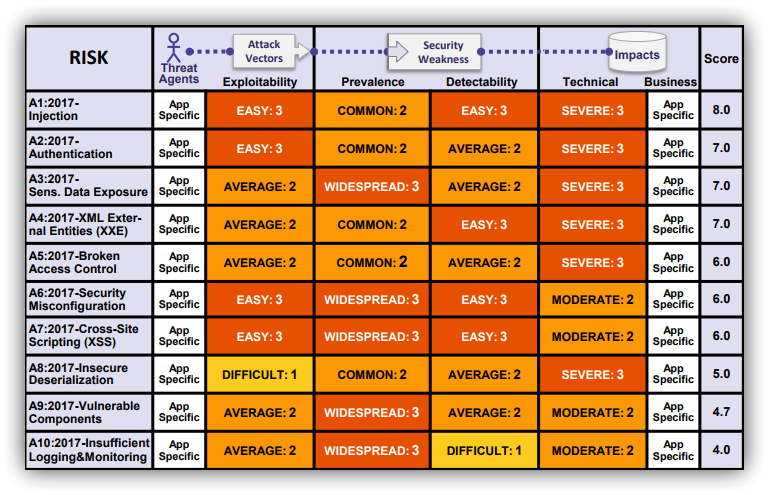
\includegraphics[width=0.75\textwidth]{includes/figures/bonus_owasp_top10_2017.png}
    \end{center}

    OWASP Top 10 - 2021:
    \begin{center}
        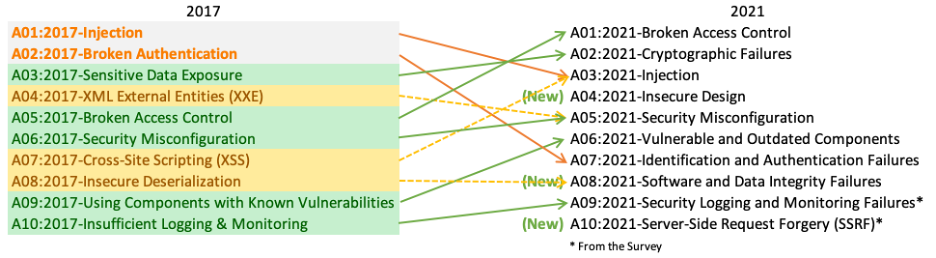
\includegraphics[width=0.75\textwidth]{includes/figures/bonus_owasp_top10_2021.png}
    \end{center}
\end{bonus}

\subsection{Injection}

\begin{defi}{Injection}
    Es gibt u. a. drei Arten von \emph{Injections}:
    \begin{itemize}
        \item SQL Injections
        \item Command Injection
        \item Code Injection
    \end{itemize}

    Injections können auftreten, wenn Eingaben von Nutzenden nicht validiert werden.
    Man darf sich nicht darauf verlassen, dass Clients Daten in dem erwarteten Format senden.

    Clientseitige Überprüfung der Daten ist sinnvoll, um versehentlich fehlerhafte Daten einzugeben.\footnote{z. B. Wenn man bei seiner E-Mail-Adresse das \texttt{\@}-Zeichen vergisst etc.}

    Um Injections zu verhindern müssen die Daten jedoch serverseitig validiert werden, da böswillige Angreifende die clientseitige Überprüfung bewusst umgehen oder über nicht vorgesehene Kanäle bzw. Verbindungen aufbauen könnten.

    \emph{cURL} ist mächtiger als ein Browser, der z. B. auf Grund von HTML-Tags gewisse Pattern voraussetzt.
\end{defi}

\begin{example}{SQL Injection (GET)}
    Erwarteter Aufruf:

    \texttt{GET http://localhost:3000/pokemon\hl{?id=4}}

    Erzeugtes SQL:
    \begin{lstlisting}[language=mysql]
        SELECT * FROM pokemon WHERE !id=4!;
    \end{lstlisting}

    \emph{Angriff mittels SQL Injection}:

    \texttt{GET http://localhost:3000/pokemon\hl{?id=4;+DROP+TABLE+pokemon}}

    Erzeugtes SQL:
    \begin{lstlisting}[language=mysql]
        SELECT * FROM pokemon WHERE !id=4; DROP TABLE pokemon!;
    \end{lstlisting}

    Hier wird anstatt einer erwarteten Anfrage die gesamte Datenbank gelöscht.
\end{example}

\begin{example}{SQL Injection (POST)}
    Erwarteter Aufruf: \\
    \texttt{POST http://localhost:3000/login} \\
    \texttt{data: \{ \enquote{user}: \enquote{admin}, \hl[\enquote{pw}: \enquote{pok3mon}] \}}

    Erzeugtes SQL\footnote{
        Kurze Erinnerung: Passwörter sollten immer verschlüsselt werden.
        Wenn eure Datenbank irgendwie an die Öffentlichkeit kommt, haben eure Nutzende deutlich weniger Probleme, da viele Menschen immer noch für verschiedene Dienste das selbe Passwort verwenden.
    }:
    \begin{lstlisting}[language=mysql]
        SELECT * FROM users WHERE username=!'admin'! AND pw=!'4b5f253b01c2d8b1f85354e0a8c619ec0f047b64'!;
    \end{lstlisting}

    \emph{Angriff mittels SQL Injection}: \\
    \texttt{POST http://localhost:3000/login} \\
    \texttt{data: \{ \enquote{user}: \enquote{admin}, \enquote{pw}: \enquote{' OR '1'='1'} \}}

    Erzeugtes SQL\footnote{Hier wird davon ausgegangen, dass das Passwort mit der Verschlüsselung \texttt{' OR '1'='1'} ist.}:
    \begin{lstlisting}[language=mysql]
        SELECT * FROM users WHERE username='admin' AND pw='' OR !'1'='1'!;
    \end{lstlisting}

    Das DBMS wird den Admin-Account zurückgeben, da \texttt{'1'='1'} immer \texttt{true} ist.

    So konnte man sich ohne richtiges Passwort als Account mit erhöhten Rechten anmelden.
\end{example}

\begin{bonus}{Abwehr von SQL Injections}
    Viele Datenbank-APIs bieten sogenannte \emph{Prepared Statements} an:

    \begin{lstlisting}[language=JavaScript]
        db.query('SELECT * FROM pokemon WHERE id = ?', [ 4 ])
        // oder
        db.query('SELECT * FROM pokemon WHERE id = :id', { 'id': 4 })
    \end{lstlisting}

    Wenn \texttt{\{ 'id': 4 \}} mitgeben wird, wird der Befehl wie gewohnt ausgeführt.

    Bei \texttt{\{ 'id': '4; DROP TABLE pokemon' \}} erkennt die API, dass dort nicht einfach nur ein Wert gesetzt wird und verhindert die Ausführung.

    Man sollte sich jedoch nicht ausschließlich darauf verlassen, dass eine API die Aufgabe erfolgreich übernimmt, sondern eventuell zusätzliche Sicherheitsmaßnahmen treffen\footnote{Escapen, Datenbank-Accounts nur mit nötigen Rechten ausstatten, etc.}.
\end{bonus}

\begin{example}{Command Injection}
    Folgende Route bekommt einen potentiell unvollständigen Dateinamen und sucht im Dateisystem nach passenden Dateien.

    \texttt{exec} führt einen Befehl lokal auf dem Server aus und benötigt ein Callback für Fehlercodes, Output (\texttt{1> stdout}) und Fehler (\texttt{2> stderr}).

    \texttt{path\_from} parsed die Ausgabe potentiell mehrerer Dateien in einen eindeutigen Pfad.

    \begin{lstlisting}[language=JavaScript]
        module.exports = express.Router()
            .post('/', (req, res) =>
                exec(`ls ../public/files -al | grep "${req.body.filename}"`, (error, stdout, stderr) => 
                    res.sendFile(path_from(stdout))
                )
            )
    \end{lstlisting}

    Erwarteter Aufruf: \\
    \texttt{POST http://localhost:3000/file} \\
    \texttt{data: \{ \enquote{filename}: \enquote{glumanda} \}}

    Erzeugter Befehl
    \begin{lstlisting}[language=bash]
        ls ../public/files -al | grep "glumanda" # Glumanda.pdf wird gefunden und versendet
    \end{lstlisting}

    \emph{Angriff mittels Command Injection}: \\
    \texttt{POST http://localhost:3000/file} \\
    \texttt{data: \{ \enquote{filename}: \enquote{'' \&\& ls \textasciitilde /.ssh/ -al | grep ''id\_rsa''} \}}

    Erwarteter Aufruf:
    \begin{lstlisting}[language=bash]
        ls ../public/files -al | grep "" && ls ~/.ssh/ -al | grep "id_rsa"
        # private ssh key wird versendet
    \end{lstlisting}
\end{example}

\begin{bonus}{Abwehr von Command Injections}
    Beim Nutzen von \texttt{exec} sollte man sehr vorsichtig sein.

    Wenn man lokal Befehle ausführen muss, sollte man sich genau überlegen was erlaubte Anfragen sind und diese \enquote{stumpf} in z. B. ein switch-Statement packen:
    \begin{lstlisting}[language=JavaScript]
        let filename
        switch(req.body.filename) {
            case 'glumanda*':
                filename = 'glumanda.pdf'
                break
            case 'pikachu*':
                filename = 'pikachu.pdf'
                break
            default:
                res.send(':(')
        }

        if (filename) { ... }
    \end{lstlisting}

    So kann die Variable trotz unzähliger Eingaben ausschließlich drei bekannte Zustände haben:
    \begin{itemize}
        \item \texttt{undefined} (default)
        \item \texttt{glumanda.pdf}
        \item \texttt{pikachu.pdf}
    \end{itemize}

    Der Node.js Server sollte ebenfalls nur mit den nötigsten Rechten laufen.
\end{bonus}

\begin{defi}{Code Injections}
    \emph{Code Injection} führt nicht nur einen Befehl auf dem Server aus, sondern bindet ganze Skripte ein.

    So werden teilweise \texttt{.js} Dateien ersetzt oder neu hinzugefügt, die dann automatisch ausgeführt werden.
\end{defi}

\subsection{Broken Auth. and Session Management}

\begin{defi}{Broken Auth. and Session Management}
    Anwendungsfunktionen, welche im Zusammenhang mit Authentifizierung und Session-Management stehen, werden häufig fehlerhaft implementiert.

    Dies erlaubt es Angreifenden, Passwörter oder Session-Tokens zu kompromittieren oder die entsprechenden Schwachstellen so auszunutzen, dass sie die Identität anderer Benutzer vorübergehend oder dauerhaft annehmen können.
\end{defi}

\begin{example}{Session über Adresszeile}
    Wenn die Session-ID aus der URL mittels GET übertragen wird, kann jeder der Session beitreten, der den Link von dem potentiellen Opfer hat.
    z. B. werden häufig Links von Shop-Seiten geteilt.

    Dies könnte man umgehen, indem man die Session-ID als Body-Parameter eines POST Requests oder als Cookie speichert.
\end{example}

\begin{example}{Session Hijacking}
    Eine erweiterte Form von \emph{Session über Adresszeile} ist es, die Reihenfolge der Schritte zu vertauschen.

    Angreifende erstellen eine Session und schicken dem potentiellen Opfer einen Link mit der Session in der Hoffnung, dass sich dieses in der Session anmeldet.
    Nun wurde sich auf beiden Clients mit der Session angemeldet.
\end{example}

\begin{example}{Nie auslaufende Sessions}
    Kritische Webseiten (z. B. einer Bank) sollten Sessions nach einem kurzen festgelegten Zeitraum löschen.

    Wenn andere Personen nun Zugriff zu dem eingeloggten Rechner erhalten, ist die Session bereits beendet und es müsste sich neu angemeldet werden.
\end{example}

\begin{bonus}{Abwehr von Broken Auth. and Session Management}
    Es wird nie eine perfekte Lösung für dieses Problem geben.

    Jedoch kann man einige Maßnahmen ergreifen, um sich bestmöglichst abzusichern:
    \begin{itemize}
        \item Mehrfaktor-Authentifizierung (beste Möglichkeit für die reine Anmeldung)
        \item Keine Standardaccounts im Werkszustand (z. B. \texttt{admin admin})
        \item Wechsel der Session-ID bei jedem Login
        \item Begrenzte Lebensdauer der Sessions
        \item Begrenzung der Fehlversuche
        \item Session-IDs über Cookies Speichern (und nicht über die URL)
    \end{itemize}

    Um immer auf einem aktuellen Stand zu sein, kann man ebenfalls vorgefertigte \emph{Session Management Frameworks} benutzen.
    Die meisten kümmern sich bereits selber um diese Probleme (zumindest wenn man sich darauf verlassen möchte).
\end{bonus}

\subsection{Sensitive Data Exposure}

\begin{defi}{Sensitive Data Exposure}
    Viele Anwendungen schützen sensible Daten\footnote{wie personenbezogene Informationen und Finanz- oder Gesundheitsdaten} nicht ausreichend.

    Angreifende können diese Daten auslesen oder modifizieren und mit ihnen weitere Straftaten begehen (Kreditkartenbetrug, Identitätsdiebstahl etc.).

    Vertrauliche Daten können kompromittiert werden, wenn sie nicht durch Maßnahmen, wie Verschlüsselung gespeicherter Daten und verschlüsselte Datenübertragung, zusätzlich geschützt werden.

    Besondere Vorsicht ist beim Datenaustausch mit Browsern angeraten.
\end{defi}

\begin{example}{Sensitive Data Exposure}
    \begin{itemize}
        \item Wichtige Daten (Passwörter, Kreditkartennummern etc.) werden im Klartext übertragen oder gespeichert.
              \begin{itemize}
                  \item z. B. bei der Nutzung von HTTP
                  \item In einem öffentlichen WLAN kann jeder die Cookies mitlesen
                  \item evtl. Backup der Daten.
              \end{itemize}
        \item Alte Verschlüsselungsalgorithmen genutzt
              \begin{itemize}
                  \item Alte Algorithmen können mit sogenannten \emph{Rainbow-Tables} geknackt werden
              \end{itemize}
        \item Verlockung des Diebstahls durch Insider
    \end{itemize}
\end{example}

\begin{bonus}{Abwehr von Broken Auth. and Session Management}
    \begin{itemize}
        \item Kein unnötiges Speichern vertraulicher Daten
        \item Verschlüsseltes Speichern von sensitiven Daten
        \item Aktuelle starke Verschlüsselungs-Algorithmen verwenden
        \item Passwörter mit Salz (und Pfeffer) versehen
        \item HTTPS verwenden
    \end{itemize}

    % \begin{wrapfigure}{r}{0.15\textwidth}
    %     \begin{center}
    %         
\includegraphics[width=0.1\textwidth]{includes/figures/nord_vpn.png}
    %     \end{center}
    % \end{wrapfigure}

    % Um sich selber in öffentlichen Netzwerken zu schützen, kann man ein VPN (Virtual Private Network) verwenden.

    % An der Stelle möchten wir euch den Sponsor dieses Spickers vorstellen.
    % Mit Nord VPN seid ihr sicher im Netz unterwegs und könnt in aller ruhe surfen.
    % Geht jetzt auf \href{https://nordvpn.com/de/pricing/}{nordvpn.com} und sichert euch mit dem Rabatt-Code \texttt{MATSE-SPICKER} 60\% Rabatt auf den drei-Jahre Plan.
\end{bonus}

\subsection{XML External Entities}

\begin{bonus}{XML External Entities}
    Viele veraltete oder schlecht konfigurierte XML-Prozessoren berücksichtigen Referenzen auf externe Entitäten innerhalb von XML-Dokumenten.

    Dadurch können solche externen Entitäten dazu eingesetzt werden, um mittels URI Datei-Handlern interne Dateien oder File-Shares offenzulegen oder interne Port-Scans, Remote-Code-Execution oder Denial-of-Service Angriffe auszuführen.
\end{bonus}

\subsection{Fehler in der Zugriffskontrolle}

\begin{defi}{Fehler in der Zugriffskontrolle}
    Häufig werden die Zugriffsrechte für authentifizierte Nutzende nicht korrekt um- bzw. durchgesetzt.

    Angreifende können entsprechende Schwachstellen ausnutzen, um auf Funktionen oder Daten zuzugreifen, für die sie keine Zugriffsberechtigung haben.

    Dies kann Zugriffe auf Account anderer Nutzenden, sowie auf vertrauliche Daten oder aber die Manipulation von Nutzungsdaten, Zugriffsrechten etc. zur Folge haben.

    Beispiele sind:
    \begin{itemize}
        \item Aufrufen authentifizierter Seiten als nicht authentifizierter Benutzender oder privilegierter Seiten als Standardbenutzender.
              Zugriff auf die API durch fehlende Zugriffskontrollen für POST, PUT und DELETE.
        \item Umgehen von Zugriffskontrollprüfungen durch Ändern der URL, des internen Anwendungsstatus, der HTML-Seite oder durch Verwendung eine API-Angriffswerkzeugs.
        \item Änderbarkeit des Primärschlüssels: Unterschieben des Schlüssels eines anderen Benutzenden, so dass das jeweilige Konto angezeigt oder bearbeitet werden kann.
        \item Fehlkonfiguration von CORS ermöglichen einen unbefugten API-Zugriffs.
    \end{itemize}
\end{defi}

\begin{example}{Insecure Direct Object References}
    Hausaufgabensystem: \\
    \url{https://www.matse.itc.rwth-aachen.de/dienste/public/show\_document.php?id=59769665} \\
    Diese URL zeigt uns die Hausaufgabe der ersten Woche in Algorithmen.
    Auf die weiteren Aufgabenblätter sollte man keinen Zugriff haben.

    Jedoch findet man relativ schnell durch erhöhen der id: \\
    \url{https://www.matse.itc.rwth-aachen.de/dienste/public/show\_document.php?id=59769673}

    Maßnahmen dagegen wäre es indirekte Objektreferenzen zu verwenden: \\
    \url{https://www.matse.itc.rwth-aachen.de/dienste/public/show\_document.php?id=1} \\
    Diese URL würde z.B. das erste Dokument anzeigen, dass für den jeweiligen Nutzenden freigeschaltet wurde.
\end{example}

\begin{example}{Missing Function Level Access Control}
    Seiten wie \texttt{http://localhost:3000/admin} sollten immer überprüfen, ob der angemeldete User ein Admin ist.
    Komplizierter wird es, wenn man mehr Abfragen halt als \texttt{user == admin}.

    Eine Lösung dafür sind Middlewares für alle Routen, die unter z. B. \texttt{/admin} liegen, die überprüfen, ob der angemeldete User Admin ist, bzw. die Rolle besitzt, die für den Zugriff notwendig ist.
\end{example}

\subsection{Sicherheitsrelevante Fehlkonfiguration}

\begin{defi}{Sicherheitsrelevante Fehlkonfiguration}
    Fehlkonfigurationen von Sicherheitseinstellungen sind das am häufigsten auftretende Problem.

    Ursachen sind:
    \begin{itemize}
        \item unsichere Standardkonfigurationen
        \item unvollständige oder ad-hoc durchgeführte Konfigurationen
              \begin{itemize}
                  \item Nicht genutzte Features sind aktiviert
                  \item Standardaccounts sind noch aktiviert (z. B. \texttt{admin admin})
              \end{itemize}
        \item ungeschützte Cloud-Speicher
        \item Fehlkonfigurierte HTTP-Header
        \item Fehlerausgaben, die vertrauliche Daten enthalten\footnote{Am besten Fehlermeldungen nicht an den Nutzenden weiterleiten.}
    \end{itemize}

    Betriebssysteme, Frameworks, Bibliotheken und Anwendungen müssen sicher konfiguriert werden und zeitnah Patches und Updates erhalten.

    Des Weiteren sollten Dev-Umgebungen wie z. B. XAMPP nicht in das Produktivsystem übernommen werden.
\end{defi}

\subsection{Cross-Site-Scripting (XSS)}

\begin{defi}{Cross-Site-Scripting (XSS)}
    \emph{Cross-Site-Scripting (XSS)} tritt auf, wenn Anwendungen nicht vertrauenswürdige Daten entgegennehmen und ohne Validierung oder Umkodierung an einen Webbrowser senden.

    XSS tritt auch auf, wenn einen Anwendung HTML- oder JavaScript-Code auf Basis von Nutzungseingaben erzeugt.

    XSS erlaubt es dem Angreifenden Scriptcode im Browser eines potentiellen Opfers auszuführen und so Benutzungssitzungen zu übernehmen, Seiteninhalte verändert anzuzeigen oder den Benutzenden auf bösartige Seiten umzuleiten.

    XSS wird in drei Arten unterteilt:
    \begin{itemize}
        \item \emph{Reflektiert} (\emph{nicht-persistent})
              \begin{itemize}
                  \item Clientdaten werden vom Server direkt in die Webseite eingebunden.
                  \item Angriff per Link auf externer Webseite oder Email
                  \item z. B. Suchanfrage
              \end{itemize}
        \item \emph{Beständig} (\emph{persistent})
              \begin{itemize}
                  \item Clientdaten werden serverseitig gespeichert und in die Webseite eingebunden.
                  \item z. B. Forum, Blog, Feedback Formular
              \end{itemize}
        \item \emph{DOM-basiert} oder \emph{lokal}
              \begin{itemize}
                  \item Ähnlich dem reflektierten Angriff (aber ohne Server)
                  \item JavaScript-Applikationen liest Clientdaten ein (z. B. als Teil der URL) und verändert entsprechend das DOM
              \end{itemize}
    \end{itemize}

    Um XSS zu verhindern kann man:
    \begin{itemize}
        \item Eingaben escapen
        \item URIs escapen
        \item JavaScript-Code escapen
        \item Nur festgelegten Code erlauben (Whitelist, CSP)
    \end{itemize}
\end{defi}

\begin{example}{Cross-Site-Scripting (XSS)}
    Erwarteter Aufruf: \\
    \texttt{GET http://localhost:3000/pokemon\hl{?search=glu}}

    \emph{Erzeugtes HTML}:
    \begin{lstlisting}[language=HTML5]
        <p>Es wird nach: ^glu^ gesucht </p>
    \end{lstlisting}

    \emph{Angriff mittels Cross-Site-Scripting}: \\
    \texttt{GET http://localhost:3000/pokemon\hl{?search=glu<script> ... </script>}}

    \emph{Erzeugtes HTML}:
    \begin{lstlisting}[language=HTML5]
        <p>Es wird nach: ^glu <script> ... </script>^ gesucht</p>
    \end{lstlisting}
\end{example}

\begin{example}{Cross-Site-Scripting (XSS)}
    Der Anmelde-Button wird dynamisch aufgebaut.

    Bei der Erstellung der Webseite wird die Methode, die diesen Button erstellt, durch eine ersetzt, die die übergebenen Daten direkt an Fremde weiterleitet.

    Für den Browser stammt der Code scheinbar von einer vertrauenswürdigen Seite.
\end{example}

\subsection{Unsichere Deserialisierung}

\begin{defi}{Unsichere Deserialisierung}
    Unsichere, weil unzureichend geprüfte Deserialisierung können zu Remote-Code-Execution-Schwachstellen führen.

    Aber auch wenn das nicht der Fall ist, können Deserialisierungsfehler Angriffsmuster wie Replay-Angriffe, Injections und Erschleichung erweiterter Zugriffsrechte ermöglichen.
\end{defi}

\begin{example}{Unsichere Deserialisierung}
    Es wird ein Cookie gesetzt, um alle Angaben zum User gespeichert werden.

    \emph{Erwarteter Cookie}: \\
    \texttt{\{ \enquote{u\_id}: \enquote{4}, \enquote{name}: \enquote{Ash}, \enquote{role}: \enquote{user}, ... \}}

    \emph{Angriff mittels unsicherer Deserialisierung}: \\
    \texttt{\{ \enquote{u\_id}: \enquote{22}, \enquote{name}: \enquote{Misty}, \enquote{role}: \enquote{\hl{admin}}, ... \}}

    Hier gibt der Angreifende an, die Rolle \enquote{Admin} zu haben, obwohl er sie potentiell nicht hat.

    Um dieses Problem zu umgehen, muss man vertrauliche Daten serverseitig speichern und alle mitgegeben Daten bei jeder Übermittlung überprüfen.
\end{example}

\subsection{Using Components with Known Vulnerabilities}

\begin{defi}{Using Components with Known Vulnerabilities}
    Komponenten wie Bibliotheken, Frameworks etc. werden mit den Berechtigungen der zugehörigen Anwendung ausgeführt.

    Wird eine verwundete Komponenten ausgenutzt, kann ein solcher Angriff von Datenverlusten bis hin zu einer Übernahme des Systems führen.

    Applikationen und APIs, die Komponenten mit bekannten Schwachstellen einsetzten, können Schutzmaßnahmen unterlaufen und so Angriffe mit schwerwiegenden Auswirkungen verursachen.
\end{defi}

\subsection{Unzureichendes Logging}

\begin{defi}{Unzureichendes Logging}
    Unzureichendes Logging und Monitoring führt zusammen mit fehlender oder uneffektiver Reaktionen auf Vorfälle zu andauernden oder wiederholten Angriffen.
    Auch können Angreifende dadurch in Netzwerken weiter vordringen und Daten entwenden, verändern oder zerstören.

    Viele Studien zeigen, dass die Zeit bis zur Aufdeckung eines Angriffs bei ca. 200 Tagen liegt sowie typischerweise durch Dritte entdeckt wird und nicht durch interne Überwachungs- und Kontrollmaßnahmen
\end{defi}

\subsection{Weitere}

\begin{defi}{Buffer Overflow}
    Ist der Puffer zu klein, werden die nachfolgenden Datenfelder im Speicher überschrieben.

    In den meisten Fällen führt dies zu einem Programmabsturz, aber bei geschickter Wahl der Overflow-Daten können eigene Funktionen in den laufenden Code geschmuggelt werden.

    Alternativ interessieren sich Angreifende für die Daten, die ein einem eigentlich nicht zugänglichen Speicher sind.
\end{defi}

\begin{bonus}{Heartbleed}
    Eine Variante von Buffer Overflow Angriffen sind Heartbleed Anfragen.

    Bei diesem Angriff fragt man bei dem Server nach der Wiederholung von gewissen Daten\footnote{z. B. damit der Server sich verifiziert oder um zu überprüfen, ob der Server noch \enquote{zuhört}}.
    Jedoch gibt man eine falsche Länge der Daten an, die potentiell nicht vom Server validiert wird.

    z. B.:

    \texttt{Client}: Wenn du mich hörst, antworte bitte mit dem 8 Zeichen Wort: \texttt{Glumanda}

    \texttt{Server}: \texttt{Glumanda}

    \texttt{Attacker}: Wenn du mich hörst, antworte bitte mit dem \hl{591} Zeichen Wort: \texttt{Glumanda}

    \texttt{Server}: \texttt{Glumanda\hl{adminpw:4b5f253b01c2d8b1f85354e0a8c619ec0f047b64}...}
\end{bonus}

\begin{defi}{Cross-Site-Request-Forgery}
    \enquote{Fälschung} einer Anfrage über einen anderen Account.
    Benutzender ist auf einer anderen Webseite autorisiert.
    Böse Webseite bindet Frame/Bild zu anderer Seite ein.

    Schutzmaßnahmen sind Tokens, die bei jedem Login generiert werden.
    Die Webseite versieht nun alle Anfragen zusätzlich mit diesem Token.
    Dieses Token kann durch POST-Request nicht von Angreifenden herausgefunden werden.
\end{defi}

\begin{example}{Cross-Site-Request-Forgery}
    \href{https://www.youtube.com/watch?v=dQw4w9WgXcQ}{https://steamcomminity.com} hat es auf einen Steam Account abgesehen.
    Dafür bindet sie das Login-Formular von \href{https://steamcommunity.com/}{https://steamcommunity.com/} ein.

    Bei der Anmeldung wird auf der \enquote{bösen} Seite der Accountname, sowie das Passwort gespeichert.
    Durch \emph{iFrames} ist der Angriff nur schwer zu erkennen.
\end{example}

\begin{defi}{Same Origin Policy}
    Die \emph{Same Origin Policy} besagt, dass nur Anfragen von einer Domäne auf gewisse Ressourcen zugreifen können.

    So kann man ausschließlich auf die Route zugreifen wenn folgendes übereinstimmt:
    \begin{itemize}
        \item Domain
        \item Subdomain
        \item Portnummer
    \end{itemize}
\end{defi}

\begin{example}{iFrames}
    \begin{center}
        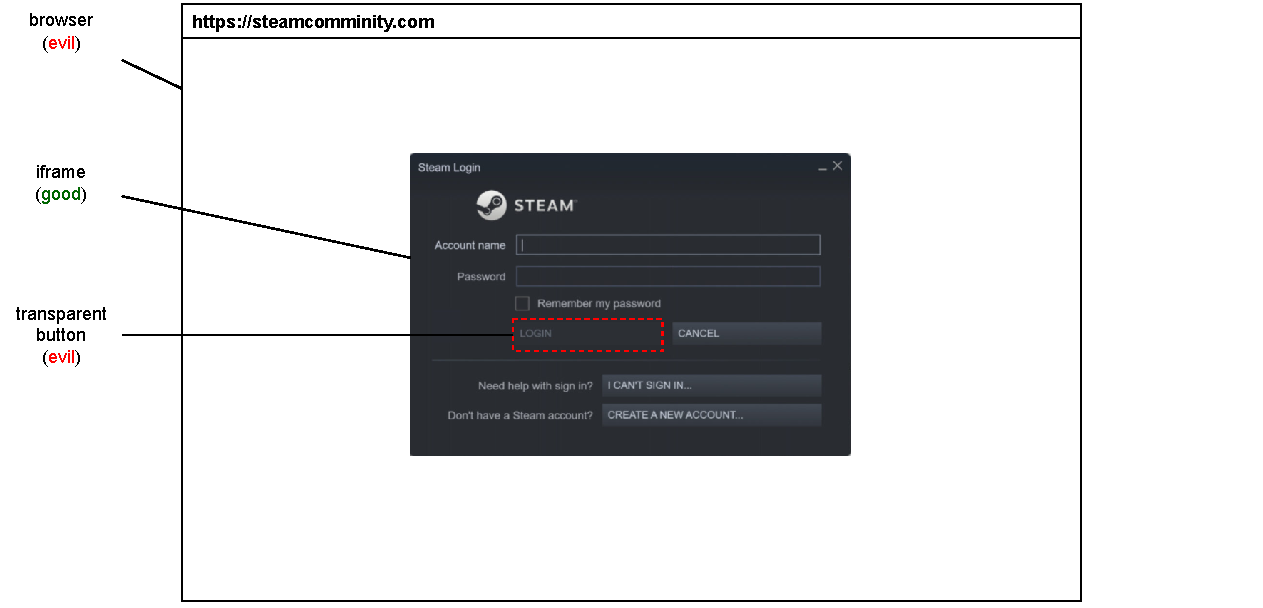
\includegraphics[width=\textwidth]{includes/figures/example_iframes.pdf}
    \end{center}
\end{example}

\begin{defi}{Insecure Design}
    Unzureichende oder fehlende Konzepte zur Zugriffskontrolle.

    Es geht nicht um die Implementierung, vielmehr um fehlerhaftes Vorgehen.

    Beispiele sind:
    \begin{itemize}
        \item \emph{Credential Recovery} mittels Fragen und Antwort.
              Obwohl dies leider immer noch üblich ist birgt dieses Vorgehen große Probleme.
              Besser vorher noch andere Mechanismen verwenden.
        \item Reservierung von Ressourcen ohne Rücksicherung, z. B. Plätze buchen ohne Bezahlung.
        \item Bots, die Lagerbestände von Angeboten leerkaufen können und diese dann woanders anbieten.
    \end{itemize}
\end{defi}

\begin{defi}{Software and Data Integrity Failure}
    Überprüfte Abhängigkeiten zu externen Ressourcen.

    Beispiele sind:
    \begin{itemize}
        \item Installation von neuen Versionen ohne Hash oder insbesondere Signatur.
              So kann beispielsweise der DSL-Router Malware enthalten.
        \item \emph{SolarWinds Orion} Attacke: Hier wurde eine Supply-Chain-Attacke gefahren, also die Schadsoftware in die Build-Chain gebracht, so dass bis zu 30.000 Systeme infiltriert werden konnten.
              Faktisch wurde also die Schadsoftware distributiert.
        \item Bots, die Lagerbestände von Angeboten leerkaufen können und diese dann woanders anbieten.
    \end{itemize}
\end{defi}

\begin{defi}{Server-Side Request Forgery (SSRF)}
    Ungeprüftes Ausführen von einer vom Benutzenden angegebenen Quelle.

    Bei dieser Attacke sendet ein Angreifender mit SSRF-Payload um Schwachstellen auszunutzen.
    Der Server antwortet dem Angreifenden wie vorgesehen, sendet jedoch sensitive Daten an den Web-Server des Angreifenden.
\end{defi}

\begin{bonus}{Weitere}
    \begin{itemize}
        \item Denial of Service (DoS)
              \begin{itemize}
                  \item Einem Dienst werden mehr Anfragen gesendet, als dieser abarbeiten kann.
                        Irgendwann ist der Dienst überlastet und stürzt ab.
              \end{itemize}
        \item Insufficient Anti-Automation
        \item Malicious File Execution
        \item Cross Frame Scripting (XFS)
        \item Cross Site Tracing
        \item Cross Site Cooking
        \item \emph{Layer 8}, der Mensch und Social Engineering
              \begin{itemize}
                  \item Auch das sicherste Passwort ist direkt geknackt, wenn der Besitzende es einem \enquote{freiwillig} mitteilt.
              \end{itemize}
    \end{itemize}
\end{bonus}

\begin{bonus}{Sicherheit garantieren}
    Man sollte von Beginn an auf Sicherheit achten.
    Beim Start der Applikation als \enquote{kleines Projekt} wird nicht an scheinbar unnötige Sicherheit geachtet.
    Selbst wenn die Applikation an Reichweite gewinnt, ist kein grundsätzliches Sicherheitskonzept vorhanden.

    Häufig wird Sicherheit eher als Feature betrachtet.
    Sicherheit ist teuer und kostet Geld.
\end{bonus}